\documentclass[a4paper,12pt]{article}
\usepackage{natbib,epsfig,rotating,longtable,url,amsmath}
\usepackage{varioref}
%% font
%%\usepackage{mathptmx}
\graphicspath{{figs/}}

\begin{titlepage}
\title{Visualisation of SPH data using SUPERSPHPLOT - v0.666 [draft only]}
\author{Daniel Price}
\end{titlepage}


\begin{document}
\maketitle
\tableofcontents

\newpage
\section{Introduction}
 Whilst many wonderful commercial software packages exist for visualising scientific
data (such as the widely used Interactive Data Language), I found that such packages
could be somewhat cumbersome for the manipulation and visualisation of my SPH data. The
main problem was that much of what I wanted to do was fairly specific to SPH (such as
interpolation to an array of pixels using the kernel) and whilst generic routines exist
for such tasks, I could not explain how they worked, nor were they
particularly fast and whilst interactive gizmos are handy, it can prove more difficult to perform the
same tasks non-interactively, as required for the production of animations. 
In fact I have found that the major
work in the visualisation of SPH data is not the image production itself but the
manipulation of data prior to plotting. Much of this manipulation makes sense
within an SPH framework (for example the interpolation provided by the kernel
and rotation of the particles for perspective).

 SUPERSPHPLOT is designed for this specific task - to use SPH tools to analyse SPH data and to make this a
straightforward task such that publishable images and animations can be obtained
as efficiently as possible from the raw data with a minimum amount of effort
from the user. I have found in the process that the development of powerful
visualisation tools has enabled me to pick up on effects present in my
simulation results that I would not otherwise have noticed (in particular the
difference between a raw particle plot and a rendered image can be substantial). Part of the goal of SUPERSPHPLOT is to eliminate the over use of particle plots as a means of representing SPH data!

\subsection{What it does}
SUPERSPHPLOT is a utility for visualisation of output from (astrophysical) simulations using the
Smoothed Particle Hydrodynamics (SPH) method in one, two and three dimensions.
It is written in FORTRAN 90/95 and
utilises PGPLOT subroutines to do the actual plotting. In particular the following
features are included:
\begin{itemize}
\item Rendering of particle data to an array of pixels using the SPH kernel
\item Cross-sections through 2D and 3D data (as both particle plots and rendered
images).
\item Fast projections through 3D data (ie. column density plots, or integration of
other quantities along the line of sight)
\item Vector plots of the velocity (and other vector quantities), including vector
plots in a cross section slice in 3D.
\item Rotation and fly-throughs (multiple cross-section slices) of 3D data.
\item Automatic stepping through timesteps, making animations simple to produce.
\item Interactive mode for detailed examination of timestep data (e.g. zooming,
rotating, plotting particle labels, working out the gradient of a line, stepping forwards/backwards
through timesteps)
\item Multiple plots on page, including option to automatically tile plots if $y-$ and $x-$ limits
are the same.
\item Plot limits can be fixed, adaptive or particle tracking. Also simple to change
axes to log, invert, square root or absolute of a quantity.
\item Exact solutions for common SPH test problems (e.g. hydrodynamic shock tubes,
polytropes).
\item Calculation of quantities not dumped (e.g. pressure, entropy)
\item Transformation to different co-ordinate systems (for both co-ordinates and
vector components).
\item Straightforward production of GIF and Postscript images which can then be
converted into animations or inserted into \LaTeX documents.
\end{itemize}

\subsection{What it doesn't do}
At the moment SUPERSPHPLOT is designed specifically for gas dynamics
simulations with SPH and has basically grown out of my visualisation needs.
However as other applications arise other features may be needed which have not
yet been included. In particular the following have not been addressed
specifically:
\begin{itemize}
\item Full 3D plotting. Visualisation in 3D is achieved by taking cross-sections
and projections through the SPH data. Similarly 2D data is plotted by means of
rendered images. At present there are no capabilities for surface plots or cubes
with faces showing cross sections and the like. However
particle plots can be plotted in a three dimensional manner using the rotation
feature (in this case 3D rotated axes/boxes are plotted appropriately).
\item It also doesn't make cappucinos.
\end{itemize}

\subsection{Version History}

\paragraph{Version 0.666}
 This is the pre-public-release (Guinea-pig) version.

\subsection{Licence}
 SUPERSPHPLOT is FREE and open source software released under the terms of the GNU General Public License (GPL). You should have received a copy of the GPL with this distribution. If not a copy may be downloaded from \url{www.gnu.org}. \c 2004 Daniel Price.

\section{Gallery}

\begin{figure}
\begin{center}
\begin{turn}{270}\epsfig{file=hyperbolic.ps,height=\textwidth}\end{turn}
\caption{A wave equation solved on SPH particles. This simulation actually resulted from some experiments for cleaning the divergence of the magnetic field in my MHD simulations. The figures show the divergence of the magnetic field in a periodic, two dimensional SPMHD simulation using a hyperbolic divergence cleaning.}
\label{fig:hyperbolic}
\end{center}
\end{figure}

\section{Getting started}
\subsection{Compiling the code}
 To compile SUPERSPHPLOT on your system you will need the following on your
system:
\begin{itemize}
\item The PGPLOT graphics subroutine library
\item A Fortran 95 compiler
\end{itemize}

\subsubsection{PGPLOT}
 The PGPLOT
graphics subroutine library is freely downloadable from
\begin{quote}
\url{http://www.astro.caltech.edu/~tjp/pgplot/}
\end{quote}
or by ftp from
\begin{quote}
\url{ftp://ftp.astro.caltech.edu/pub/pgplot/pgplot5.2.tar.gz}
\end{quote}
however check to see if it is already installed on your system (if so, the libraries are
usually located in /usr/local/pgplot). For details of the actual plotting subroutines
used by the SUPERSPHPLOT source code, you may want to refer to the PGPLOT userguide:
\begin{quote}
\url{http://www.astro.caltech.edu/~tjp/pgplot/contents.html}
\end{quote}


\subsubsection{Fortran 90/95 compilers}
 By now, many Fortran 90/95 compilers exist. Amongst the most popular commercially
available ones are perhaps the NAG Fortran compiler and the Intel Fortran Compiler (ifc). However, the
g95 project has produced a free compiler, which is downloadable from:
\begin{quote}
\url{http://www.g95.org}
\end{quote}
and which successfully compiles SUPERSPHPLOT. Another, apparently unrelated project is located at
\begin{quote}
\url{http://gcc.gnu.org/fortran}
\end{quote}
however this compiler is not fully implemented and therefore does not as yet compile SUPERSPHPLOT.

\subsubsection{Makefile options}

 In the Makefile, you will need to set the FORTRAN compiler and flags to your local version, e.g..
\begin{verbatim}
F90C = g95
F90FLAGS = -O
\end{verbatim}
 Secondly the compiler must be able to link to the PGPLOT and X11 libraries on
your system. As a first attempt try using:
\begin{verbatim}
LDFLAGS = -lpgplot -lX11
\end{verbatim}
If that works at a first attempt, take a moment to think several happy thoughts about your system
administrator. If these libraries are not found, you will need to enter the
library paths by hand. On most systems this is something like:
\begin{verbatim}
LDFLAGS = -L/usr/local/pgplot -lpgplot -L/usr/X11R6/lib -lX11
\end{verbatim}
(assuming the PGPLOT libraries are in the /usr/local/pgplot directory and the
X11 libraries are in /usr/X11R6/lib). If this does not work, try using the
\verb+locate+ command to find the libraries on your system:
\begin{verbatim}
locate libpgplot
locate libX11
\end{verbatim}
 If, having found the PGPLOT and X11
libraries, the program still won't compile, it is usually
because the PGPLOT on your system has been compiled with a different compiler to
the one you are using. A first attempt is to try using the g2c libraries
\begin{verbatim}
LDFLAGS = -L/usr/local/pgplot -lpgplot -L/usr/X11R6/lib -lX11 -lg2c
\end{verbatim}
If the PNG drivers are incorporated into the PGPLOT installation, the \verb+-lpng+ libraries must also be added.
Failing that, ask your system administrator(!) or simply download your own copy of
the PGPLOT libraries and make sure it is compiled with the same compiler as you
are using to compile the SUPERSPHPLOT source code.

\subsection{Environment variables}
 Several useful environment variables can be set for PGPLOT and several of them
are very useful for SUPERSPHPLOT. In a tcsh shell type:
\begin{verbatim}
setenv PGPLOT_DEV /xwin
setenv PGPLOT_BACKGROUND white
setenv PGPLOT_FOREGROUND black
\end{verbatim}
The first command sets the default device to the X-window, rather than the /null
device. The latter two commands set the background and foreground colours of the
plotting page. Note that these environment variables should be set \emph{before}
invoking supersphplot (it is simplest to set them upon starting the shell by placing
them in your .tcshrc or bash/sh equivalent file). For other environment
variables which can be set, refer to the PGPLOT user guide.

\subsection{System dependent routines}
 System dependent subroutines are interfaced in a separate \verb+system+ module in the file \verb+system_unix.f90+.
At present the only calls to these routines are made from \verb+supersphplot.f90+ which
reads the run name(s) from the command line (see \S\vref{sec:commandline}). A standardised format for performing this
task is included in the standards for the next release of Fortran (Fortran 2003),
however in the meantime the calls in the \verb+system+ module may require some adjustment depending on the
particular system you are compiling the code on. The program is still fully
functional without this call working, but it does make things convenient (in particular it means that
SUPERSPHPLOT can be invoked using wildcards ($*,?$) in filenames).

\section{Reading data}
 The most important part is getting SUPERSPHPLOT to read your data format. I
have supplied subroutines for reading output from the publically available
GADGET code (\verb+read_data_gadget.f90+) and also for Matthew Bate's SPH code
(\verb+read_data_mbate.f90+) which is widely used in the UK. Another example of a
data read which I use is given in \verb+read_data_dansph.f90+.
 Since the specifics of the data read can
vary between codes, I recommend examining these subroutines before writing your
own version. Further details on writing your own subroutine are given in
appendix~\ref{sec:writeyourown}

 Using one of the subroutines provided, invoke SUPERSPHPLOT with the name of the data
file on the command line, e.g.
\begin{verbatim}
supersphplot myrun
\end{verbatim}
With multiple filenames on the command line, ie.
\begin{verbatim}
supersphplot myrun1 myrun2 myrun3
\end{verbatim}
or simply
\begin{verbatim}
supersphplot myrun*
\end{verbatim}
files will be read consecutively in the order that they are given.

\section{A brief tour...}
After a successful data read, the menu should appear as something like the
following:
\begin{verbatim}
 You may choose from a delectable sample of plots
 -------------------------------------------------------
  1) x                     7) particle mass
  2) y                     8) u
  3) z                     9) \gr
  4) v\dx                 10) pressure
  5) v\dy                 11) entropy
  6) v\dz                 12) h
 -------------------------------------------------------
 13) multiplot [  4 ]      m) set multiplot
 -------------------------------------------------------
  d(ata) i(nteractive) p(age) o(pts) l(imits) h(elp)
  r(ender) v(ector) x(sec/rotate) s(ave) q(uit)
 -------------------------------------------------------
Please enter your selection now (y axis or option):
\end{verbatim}
The simplest plot is of two quantities where only one is a coordinate, for
example
\begin{verbatim}
Please enter your selection now (y axis or option): 9
(x axis) (<cr>=1): 1
 Graphics device/type (? to see list, default /xwin): /xw
\end{verbatim}
 A full list of available graphics devices is given in the PGPLOT user guide.
Some of the most useful devices are given in table \ref{tab:devices}. In the
above we have selected the x-window which means that the output is sent to the
screen, producing the graph shown in Figure \ref{fig:swave1D}.
\begin{table}[h]
\centering
\begin{tabular}{|l|l|}
\hline
\verb+/xw+, \verb+/xwin+ & X-Window (interactive) \\
\verb+/ps+ & Postscript (landscape) \\
\verb+/vps+ & Postscript (portrait) \\
\verb+/cps+ & Colour Postscript \\
\verb+/gif+ & GIF \\
\verb+/png+ & PNG (if installed) \\
\verb+/null+ & null device (no output) \\
\hline
\end{tabular}
\caption{Commonly used graphics devices available in PGPLOT}
\label{tab:devices}
\end{table}

\begin{figure}
\centering
\caption{example plot}
\end{figure}
 Plot settings are controlled via the menu options and are described below. 


\section{Menu options}
 The program options may be changed in a series of submenus. The defaults for all of
these options are initially set in the subroutine defaults\_set. The options set using
the submenus can be saved using the (s)ave option from the menu. This saves all of
the current options to a file called `defaults' in the current directory, which is
automatically read upon starting supersphplot the next time. This file is written using
the namelist formatting option provided by Fortran 90. An alternative way of setting
options is to edit this file directly prior to invoking the program, referring to the
variable list given in \S\ref{sec:variables} of this user guide. 

\subsection{set (m)ultiplot}
 The multiplot option enables plotting of several different plots on the same
physical page. Plots with the same $x-$ and $y-$ axes are tiled if the tiling
option from the (p)age options menu (\S\vref{sec:optionspage}) is set. Each plot
can have independent $x-$ and $y-$ axes as well as a different rendering (cross
section or projection) and/or vector plot. For rendered plots plotting of
contours can be turned on/off between plots and for cross sections the position of
the cross section can also be changed between plots. An alternative method for
specifying a multiplot is to edit the \verb+defaults+ file directly prior to
starting SUPERSPHPLOT.

\subsection{(d)ata options}
These options relate to the data read and are as follows:
\begin{enumerate}
\item \textbf{read new data}. Read new data, using a different runname.
\item \textbf{change number of timesteps read}. Set timestep number to start
reading from, timestep number to stop reading from and the frequency of
timesteps to read (e.g. every two steps). This can also be changed interactively in
interactive mode.
\end{enumerate}

\subsection{(i)nteractive mode}
 The menu option turns on/off interactive mode. With this option turned on and
an appropriate device selected (ie. the X-window, not /gif or /ps), after
each plot the program waits for specific commands from the user. With the cursor
positioned anywhere in the plot window (but not outside it!), commands can be invoked using the
following keystrokes:

\begin{tabular}{rcp{0.75\textwidth}}
 h & : & display/hide help text \\
 left click & : & select area to zoom in on \\
 + & : & zoom in by 10\% with plot centred on current cursor position \\
 - & : & zoom out by 10\% with plot centred on current cursor position \\ 
 s & : & save the current plot limits for all timesteps \\
 p & : & label the particle closest to the cursor position \\
 l & : & draw a connecting line between the closest particle and a second
 particle (to be selected) and calculate the slope of this line. \\
 r & : & replot the current plot. \\
 space & : & advance to next timestep \\
 right click & : & go back to previous timestep \\
  1,2,3..9 & : & on space/right click, jump forward/backwards by $n$ timesteps \\
  q & : & quit plotting 
\end{tabular}

 NB: If the multiplot option has been used, the timestep changing commands only
take effect on the last plot per timestep. Many more commands could be added to
the interactive mode, limited only by your imagination. Please send me your suggestions!

\subsection{(p)age options}
\label{sec:optionspage}
 This submenu contains options relating to the PGPLOT page setup. The options are as follows:
\begin{enumerate}
\item \textbf{toggle page change}. (default=on) When turned off, no new page is
created between plots. This means that consecutive timesteps are plotted
directly on top of one another. For particle plots this can be used to trace the
position of the particles as they evolve in time.
\item \textbf{toggle axes}. Changes the appearance of the axes. The variable is
the same as the AXIS variable used in the call to PGENV in the standard PGPLOT
routines, except that I have also added the $-3$ option. The options are
as follows:

\begin{tabular}{rcp{0.8\textwidth}}
-3 & : & same as AXIS=-1, but also draw tick marks; \\
 -2 & : & draw no box, axes or labels; \\
 -1 & : & draw box only; \\
  0 & : & draw box and label it with coordinates; \\
  1 & : & same as AXIS=0, but also draw the coordinate axes (X=0, Y=0); \\
  2 & : & same as AXIS=1, but also draw grid lines at major increments of the coordinates;
\end{tabular}

\item \textbf{change paper size}. Sets the size of the plotting page.
\item \textbf{change plots per page}. Changes the number of plots on each
physical page.
\item \textbf{toggle plot tiling}. When set, plots with more than one plot on
the page and the same $y-$ and $x-$ axes are automatically tiled together.
\item \textbf{adjust title position}. Adjusts the position of the title on
each plot. To turn off plot titling, set the position outside the viewport (ie.
enter some large numbers). For details of plot titling see \S\vref{sec:title}
\item \textbf{adjust legend position}. Adjusts the position of the legend on
each plot. Again, to turn off the legend, set the position outside of the
viewport (ie. enter some large numbers). To customise the legend see
\S\vref{sec:legend}
\item \textbf{toggle animate}. When set, this turns off the prompting given
before the page is changed. Does not apply in interactive mode, where the page
changing can be controlled using the mouse. 
\end{enumerate}

\subsection{particle plot (o)ptions}
 These options relate to pure `particle plots'. The options are as follows:
\begin{enumerate}
\item \textbf{toggle plot line}. When set, this option plots a line connecting the particles
in the order that they appear in the data array. Useful mainly in one dimension, although can give an indication of the
relative closeness of the particles in memory and in physical space in higher dimensions.
\item \textbf{toggle plot average line}. Bins the particles into $nbin$ bins along the
$x-$axis, calculates the average value of the $y-$axis quantity in each bin and
plots a line through these points. 
\item \textbf{toggle label particles}. This option prints the number of each particle
next to its position on the plot (for all particles). Primarily useful for debugging neighbour finding
routines. An alternative is to use the `p' option in interactive mode.
\item \textbf{circles of interaction}. On coordinate plots this option plots a circle of
radius $2h$ around either all particles or on up to 10 selected individual particles. 
This is primarily useful in debugging neighbour finding routines. On
non-coordinate plots an error bar of length $2h$ in either direction is plotted
in the direction of the coordinate axis.
\item \textbf{plot ghosts/sinks}. Enables particles of certain types only to be plotted
(e.g. dark matter particles only, gas particles only or both).
\item \textbf{change graph markers}. This option sets the PGPLOT marker used for each
type of particle in the particle plots. The list of markers is given in the
PGPLOT user guide and is also listed in Appendix \ref{sec:pgplotmarkers}. 
\item \textbf{toggle cross section/projection}. In three dimensions this determines
whether to all the particles projected onto the plane or to plot particles only
in a given co-ordinate range. Also applies to rendered and vector plots.
\item \textbf{change co-ordinate systems}. This feature transforms the particle
co-ordinates and vector components into non-cartesian co-ordinate systems. This
is useful for simulation data which has a particular symmetry associated with it
(e.g. for accretion disc simulations, the components of velocity in the radial
and azimuthal directions can be plotted). Note that this option does \emph{not} change
the co-ordinate system used on rendered plots, as this would mean that the interpolation using the SPH
kernel would not be correct.  
\item \textbf{toggle exact solution}. The following exact solutions are provided
\begin{itemize}
\item Hydrodynamic shock tubes (Riemann problem)
\item Spherically-symmetric sedov blast wave problem. This
\item Polytropes (with arbitrary $\gamma$)
\item One dimensional toy stars. This is a particularly simple test
problem for SPH codes described in \citet{mp04}.
\item Linear wave. This simply plots a sine wave of a specified amplitude, period and
wavelength on the plot specified.
\item MHD shock tubes (tabulated). These are tabulated solutions for 7 specific MHD
shock tube problems.
\item Exact solution from a file. This option reads in an exact solution from the
filename input by the user, assuming the file contains two columns containing the $x-$ and $y-$ co-ordinates of
an exact solution to be plotted as a line on the plot specified.
\end{itemize}
Details of the calculation of the exact solutions and examples of their output are
given in Appendix \ref{sec:exact}. Note that the PGPLOT call to plot the line is included in the
exact solution subroutine so as to provide flexibility should an exact solution require
multiple lines on the page / different line styles etc. (although none of those
provided do).
\end{enumerate}


\subsection{plot (l)imits}
\label{sec:optionslimits}
 The options for plot limits are as follows:
\begin{enumerate}
\item \textbf{toggle fixed/adaptive limits}. With limits set to adaptive, plot
limits are minimum and maximum of quantities at current
timestep. However, the co-ordinate limits are not adapted in the case of
rendered plots. With fixed limits, the plot limits retain their default values
for all timesteps.
\item \textbf{set manual limits}. Manually set the limits for each column of
data.
\item \textbf{x-y limits track particle}. Co-ordinate limits are centred on the
selected particle for all timesteps, with offsets as input by the user. This
effectively gives the `Lagrangian' perspective.
\item \textbf{zoom in/out}.
\item \textbf{apply transformations (log10,1/x)}.
\item \textbf{save current limits to file}. Saves the current values of the
limits calculated from the data read or set manually using option (2) to the
file `rootname.limits' where rootname is the name of the current run. This file
is automatically read upon the next invocation of supersphplot. The limits apply
only when fixed limits are set.
\item \textbf{re-read limits file}. Re-reads the plot limits from the
`rootname.limits' file. This means that the limits contained in this file can be
manually changed by the user whilst the program is still running.
\end{enumerate}

\subsection{(r)endering options}
\begin{enumerate}
\item \textbf{change number of pixels}. Set the number of pixels along the
$x-$axis. Pixels are assumed to be square such that the number of pixels along
the $y-$axis is determined by the aspect ratio of the current plot.
\item \textbf{change colour scheme}. Changes the colour scheme used on rendered
images. A demonstration of all the colour schemes can be also be invoked from
this menu option. Setting the colour scheme to zero plots only the contours of
the rendered quantity (assuming that plot contours is set to true). The colour
schemes given are as follows:

\begin{tabular}{rcp{0.8\textwidth}}
  0 & : & contours only \\
  1 & : & greyscale \\
  2 & : & red \\
  3 & : & ice blue \\
  4 & : & rainbow \\
  5 & : & frog monster
\end{tabular}

User contributed colour schemes are eagerly invited (see the subroutine
`colour\_set' for details on how to do this).
\item \textbf{toggle cross section/projection}. For 3D data, toggles whether to
plot the rendered quantity integrated along the line of sight (projection) or in
a particular cross section along the line of sight. For 2D data setting the
cross section option gives arbitrary 1D cross sections through 2D data. Also applies to vector and plots.
\item \textbf{toggle plot contours}. Determines whether or not to plot contours
in addition to the rendered quantity.
\item \textbf{change number of contours}. Sets the number of contours to be
plotted. 
\item \textbf{toggle colour bar}. Determines whether or not to plot the colour
bar on rendered images.
\end{enumerate}

\subsection{(v)ector plot options}
\begin{enumerate}
\item \textbf{change number of pixels}. Set the number of pixels along the
$x-$axis to be used in the vector plots. As in the rendered images, pixels are assumed to be square such that the number of pixels along
the $y-$axis is determined by the aspect ratio of the current plot.
\item \textbf{toggle particle plotting if no rendering}. If no rendered quantity
is set, toggles whether or not to plot the particles in addition to the vector
plot.
\item \textbf{toggle background/foreground colour}. Determines whether or not to
plot the vector arrows in the current background or foreground colour (by
default these are white and black respectively). This must
be user determined to give the best contrast between the vector arrows and the
rendered image.
\end{enumerate}

\subsection{(s)ave, (h)elp, (q)uit}
 The (s)ave options saves the default options to a file called `defaults' in the
current directory which is read automatically upon the next invocation of
supersphplot. The (h)elp option simply expands the text for the options menus (I
may add to this soon). (q)uit, unsurprisingly, quits. Typing a number greater than the number of
data columns also exits the program (e.g. I often simply type 99 to exit).

\section{Other features}

\subsection{Plot titles}
\label{sec:title}
 Plots may be titled individually by creating a file called \verb+titlelist+ in
the current directory, with the title on each line corresponding to the position
of the plot on the page. Thus the title is the same between timesteps unless the
steps are plotted together on the same physical page. Leave blank lines for
plots without titles. For example, creating a file called \verb+titlelist+ in
the current directory, containing the text:
\begin{verbatim}
plot one
plot two
plot three
lucky me

oops
\end{verbatim}
and positioning the title using the default options, produces the titles shown
on the graph in Figure~\ref{fig:titleexample} (where there are 6 plots on the physical page).

\begin{figure}
\centering

\caption{Example use of plot titles}
\label{fig:titleexample}
\end{figure}

\subsection{Plot legends}
\label{sec:legend}
 Legends are a tricky business.


\subsection{Rotation}
 Rotation is achieved by tranforming to spherical co-ordinates, incrementing the
azimuthal and tilt angles appropriately and transforming back to cartesians.
An example of rotation of two dimensional data is shown in
Figure~\ref{fig:examplerot2D} 
\begin{figure}
\centering

\caption{Example of plot rotation in 2D}
\label{fig:examplerot2D}
\end{figure}

An example of the rotation of 3D data to give a 3D particle plot is shown in
Figure \ref{fig:examplepartrot3D}. Note the axes which have been rotated and
plotted accordingly. 
\begin{figure}
\centering

\caption{Example of particle plot rotation in 3D}
\label{fig:examplepartrot3D}
\end{figure}

\subsection{Flythru}

\subsection{Co-ordinate transformations}


\subsection{Power spectrums (1D only)}
 In one dimension an extra plot item appears
in the data menu which takes a power spectrum (in space) of a particular
variable defined on the particles. Upon selection the user is prompted for
various settings before plotting the power spectrum. For data defined on
irregularly distributed particles, there are two methods for taking the power
spectrum: Either to interpolate to an even grid and use a Fourier
transform or to use a method for calculating a periodogram of
irregularly sampled data which can have significant advantages over
interpolation. Algorithms for both of these methods have been
implemented. For the first, the SPH data is interpolated to a one dimensional
grid using the kernel via the \verb+interpolate1D+ subroutine before calculating the (slow!) fourier
transform in \verb+powerspectrum_fourier+. For the second, an algorithm due to
Lomb and \citet{scargle81} described in \citet{numericalrecipes} is
used\footnote{Note that the subroutines given in \citet{numericalrecipes} have
\emph{not} been used as they are not free software.},
located in the subroutine \verb+powerspectrum_lomb+. The actual plotting is done
in the subroutine \verb+plot_powerspectrum+. An example of this feature is shown
in Figure~\ref{fig:powerspectrum_lomb}, where a power spectrum of a given
spectral index has been defined on the particles as an initial condition. The
plot shows the velocity variable given the initial power spectrum and the power
spectrum calculated via the Lomb periodogram.
\begin{figure}
\centering

\caption{Example of one dimensional power spectrum using the Lomb periodogram}
\label{fig:powerspectrum_lomb}
\end{figure}

 It should be stressed, however, that \emph{neither} of the subroutines for
calculating the power spectrum is particularly fast and have \emph{only} been included as a preliminary feature
since I have used them once or twice in one dimensional simulations where speed
is not an issue. The algorithms are fairly simple to extend to multidimensional
data, although faster implementations would be needed (such as a Fast
Fourier Transform routine).


\section{Interpolation routines}

\subsection{Two dimensional interpolation}
\subsubsection{Rendering of 2D data}
 For a contour or rendered plot of a scalar quantity $\phi$ we
interpolate from the particles to an array of pixels using the SPH summation
interpolant. In two dimensions the interpolant is simply
\begin{equation}
\phi(x,y) = \sum_b m_b \frac{\phi_b}{\rho_b} W(x - x_b, y-y_b, h_b)
\end{equation}
where the summation is over contributing particles and $W$ is the standard cubic spline kernel, given by
\begin{equation}
W(q) = \frac{\sigma}{h^\nu}\left\{ \begin{array}{ll}
1 - \frac{3}{2}q^2 + \frac{3}{4}q^3, & 0 \le q < 1; \\
\frac{1}{4}(2-q)^3, & 1 \le q < 2; \\
0 & q \ge 2 \end{array} \right.
\end{equation}
where $q = \vert {\bf r}_a - {\bf r}_b \vert / h$, $\nu$ is the number of spatial
dimensions and the normalisation constant $\sigma$ is given by $2/3$, $10/(7\pi)$ and $1/\pi$ in
1, 2 and 3 dimensions respectively.

In three dimensions, we must either take a cross section or a projection
through the data.

\subsection{Projections through 3D data}

\subsection{Cross sections}

\subsubsection{Cross sections of 3D data}
 A cross section can be taken of SPH data by summing the
contributions to each pixel in the cross section plane from all particles within
$2h$ of the plane. This is done in the subroutine interpolate\_3D\_fastxsec. In
this case the cross section is always at a fixed value of the third co-ordinate
(ie. for xy plots the cross section is in the z direction). Oblique cross
sections can be taken by rotating the particles first.

 A routine is also provided to do cross sections of two dimensional data (ie. take one dimensional
cross sections) (interpolate2D\_xsec). In this case the cross-section line can be arbitrarily
specified. I will hopefully write an interactive version of this one day.
\begin{figure}
\begin{center}
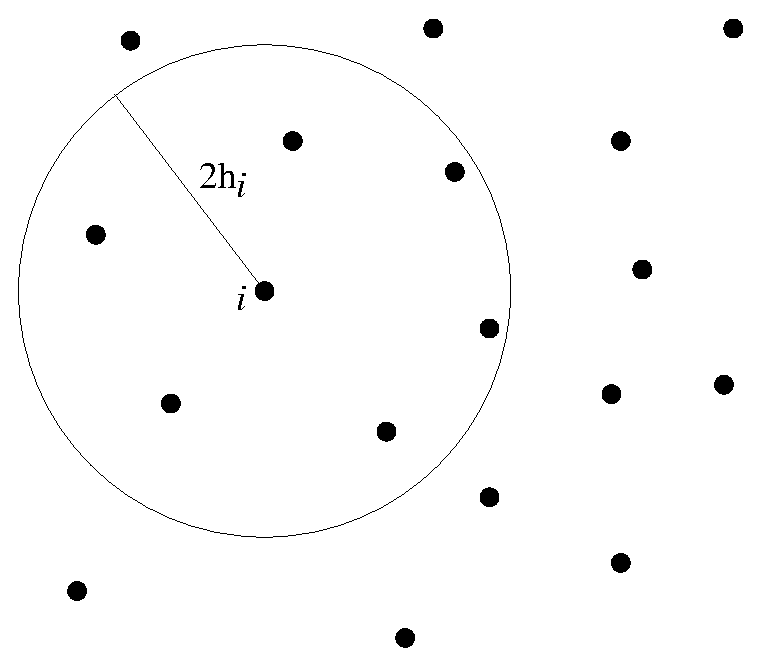
\epsfig{file=xsec3D.eps,width=0.5\textwidth}
\caption{Computation of a two dimensional cross section through 3D data}
\label{fig:xsec3D}
\end{center}
\end{figure}


\subsubsection{Cross sections of 2D data}
The cross-sectioning algorithm for 2D data (giving a 1D line) is slightly
different, in that it also works for oblique cross sections. The
cross-sectioning is done in the subroutine interpolate2D\_xsec. The cross
section is defined by two points (x1,y1) and (x2,y2) through which the line
should pass. These points are converted to give the equation of the line in the
form
\begin{equation}
y = mx + c
\end{equation}
This line is then divided evenly into pixels to which the particles
may contribute. The contributions along this line from the particles is computed
as follows: 

 For each particle, the points at which the cross section line intersects the
smoothing circle are calculated (illustrated in Figure \ref{fig:xsec2D}). The
smoothing circle of particle $i$ is defined by the equation
\begin{equation}
(x-x_i)^2 + (y-y_i)^2 = (2h)^2
\end{equation}
The x-coordinates of the points of intersection are the solutions to the quadratic equation
\begin{equation}
(1 + m^2) x^2 + 2 (m (c - y_i) - x_i) x + (x_i^2 + y_i^2 - 2cy_i + c^2 - (2h)^2)= 0
\end{equation}
For particles which do not contribute to the cross section line, the determinant
is negative. For the particles that do, it is then a simple matter of looping
over the pixels which lie between the two points of intersection, calculating
the contribution using the SPH summation interpolant
\begin{equation}
\phi = \sum_b m_b \frac{\phi_b}{\rho_b} W(x - x_b, h_b)
\end{equation}

\begin{figure}
\begin{center}
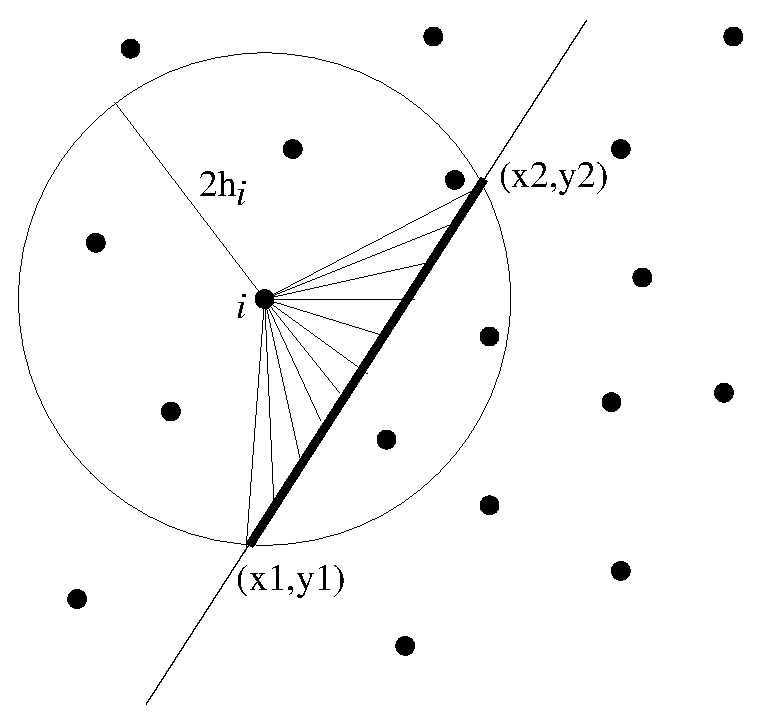
\epsfig{file=xsec2D.eps,width=0.5\textwidth}
\caption{Computation of a one dimensional cross section through 2D data}
\label{fig:xsec2D}
\end{center}
\end{figure}
 
 An example of a 1D cross section through 2D data is shown in Figure
\ref{fig:xsec2Dexample}.
\begin{figure}
\begin{center}
%%\begin{turn}{270}\epsfig{file=xsec2Dexample.ps,height=\textwidth}\end{turn}
\label{fig:xsec2Dexample}
\end{center}
\end{figure}

 In principle a similar method could be used for oblique cross sections
through 3D data. In this case we would need to find the intersection
between the smoothing sphere and the cross section plane. However
in 3D it is simpler just to rotate the particles first and then take
a straight cross section as described above.

\subsection{Projections}


\subsection{Vector plots}
 


\section{FAQS: How do I...}

\subsection{Read/process my data into images without having to answer prompts?}
 Firstly edit the settings in the \verb+defaults+ file in the current
directory (created by doing a `save defaults' from the main menu) before invoking SUPERSPHPLOT. An explanation of the variables used in this
file is given in Appendix~\ref{sec:variables}. 

 Having edited the defaults file, the simplest way of running SUPERSPHPLOT
non-interactively is to write a small shell script which runs SUPERSPHPLOT
and answers the prompts appropriately. Something like the following should work:
\begin{verbatim}
#!/usr/bin/tcsh
cd plot
supersphplot myrun* << ENDINPUT
2
1
8
0
mypostcript.ps/ps
q
ENDINPUT
\end{verbatim}
which would plot the data in columns 2 and 1 and render the data in column 8 with
output to file \verb+mypostscript.ps+.

\subsection{Calculate additional quantities?}
 Additional quantities are calculated in the subroutine \verb+calc_quantities+,
in which it should be a simple matter to add your own.
If the calculated quantity is to be used elsewhere (for example in an exact
solution), an indicator should be created for its position in the data array
(e.g. the integer variable \verb+ih+ refers to the position of the smoothing
length in the data array). It is also preferable to indicate those quantities
from which the new quantity is calculated, so that no error will occur if they
are not present.

\subsection{What about boundaries? How does the rendering work near a boundary?}
 Usual practise in SPH simulations near boundaries is
to introduce ghost particles which mirror the real particles. SUPERSPHPLOT does not
explicitly setup any ghost particles but will use any that are present in the data
(specified using \verb+labeltype = 'ghost'+ in the \verb+read_data+ subroutine and
then specifying the number of particles of this type). Ghost particles contribute
to the rendering calculations but not to the determination of the plot limits. Note,
however, that SUPERSPHPLOT does \emph{not} set up ghost particles itself, as this may depend
on the type and location of the boundary. Thus if your simulation uses ghost particle
boundaries, the ghost particles should be dumped alongside the gas particles in the
output file so that their positions, masses, densities and smoothing lengths can be
read into SUPERSPHPLOT and used to render the image appropriately.

\subsection{Use special characters in the plot labels?}
 Several of the examples shown in this manual use special characters (such as
the $\int$ character) in the plot labels. The PGPLOT user guide explains how to do
this, but the basic idea is that PGPLOT uses escape sequences to plot special
characters. For example to plot the greek letter $\rho$ we would use
\begin{verbatim}
label = 'this would print the greek letter \gr'
\end{verbatim}
where \verb+\gr+ is the PGPLOT escape sequence for $\rho$. For other
characters the escape sequence is given by a number. For example for the integral 
\begin{equation}
\int v_x \mathrm{dx}
\end{equation}
we would use
\begin{verbatim}
label = '\(2268) v\d x \u dx'
\end{verbatim}
where \verb+\(2268)+ is the escape sequence for the integral sign. The
\verb+\d+ indicates that what follows should be printed as subscript and
\verb+\u+ correspondingly indicates a return to normal script (or from normal script to
superscript). All of the escape sequences for special characters are listed in
the appendix to the PGPLOT user guide.
\begin{quote}
 WARNING: Note that the use of escape characters can be compiler dependent and
 may not therefore work on all compilers.
\end{quote}

\subsection{Customise the legend?}

\subsection{Make movies?}
 At the PGPLOT device prompt
\begin{verbatim}
Graphics device/type (? to see list, default /xwin):
\end{verbatim}
choose \verb+/gif+ or \verb+/vgif+ (some installations of PGPLOT may also have \verb+/png+
installed). The images will then be written as \verb+.gif+ files which can then be easily compiled
together to form an animation. Under unix the \verb+gifmerge+ command (if installed) is a simple way
of making a single animated gif file out of a series of gif images. Animated gifs are robust but
require large amounts of memory to run at any reasonable speed. However many software packages exist
for converting animated gifs into other, more compressed formats (such as the windows .avi format or
under unix the .fli format\footnote{Note that MPEG is a particularly poor choice for simulation data}). One such package is the
\verb+convert+ command included as part of the GIMP (Gnu Image Manipulation Package) toolkit.
For presentations the windows .avi format is a good choice, although codecs for conversion are a
little harder to come by. Under windows the commercially available \verb+videomach+ program is one
such tool as well as several Microsoft products.

 Another tool under unix is the \verb+fbm2fli+ package, which will take a series of .gif or .png files and
convert them into a .fli animation (which can be played, for example by the \verb+xanim+ tool). This
format is great for animations of simulations but as yet does not import into powerpoint and the like.

\section{User contributions / Wishlist for future improvements}
 Please contribute!! Any user contributions and/or suggestions would be greatly
appreciated. The following in particular would be very useful:

\begin{itemize}
\item Exact solutions for your favourite test problem(s). It would be great to
build a library of user-contributed exact solutions.
\item Data analysis tools (e.g. fourier transforms / statistical analysis /
algorithms for finding binary stars etc) which could be incorporated.
\item New visualisation techniques (e.g. an isosurfacing routine for SPH, better
vortex line tracing).
\item More colour schemes (see \verb+colour_set.f90+ for how to do this)
\item Pretty pictures! If you happen to plot some of your data and spend the
next several minutes marvelling at how astoundingly beautiful it all looks, please send
me a copy (either ps, gif or a movie) to add to the gallery and a few lines
describing the simulation.
\end{itemize}


If you wish to send me subroutines or snippets of (Fortran only!) code for doing any of the above or
more, please also send me a \LaTeX file
documenting the subroutine similar to the documentation given in this user guide.
Also, please, please comment your code clearly so that others can figure out
what it does and try to catch as many errors as possible so that the whole
program is robust.  One thing I have avoided doing is to use any SPH
routines which explicitly require finding neighbours, to avoid introducing treecodes and
the like and to keep the program independent of any particular implementation of
SPH. An example of a
routine would be to find the div/curl of a vector quantity using
the SPH summation.

Contributions, comments and inevitable bug fixes
should be sent to:
\begin{verbatim}
dprice@ast.cam.ac.uk
\end{verbatim}
although check that this email address is current because I am still a postdoc!

\subsection{Known limitations / issues}
Here is a partial to do list or things which currently conflict:
\begin{itemize}
\item rotation settings override limits transformations on co-ordinate plots
\item exact solutions cannot be transformed yet
\item Does not yet handle non-cartesian input data
\end{itemize}

\section*{Acknowledgements}
 Several of the routines were developed from ideas used by Matthew Bate. The
polytrope exact solution is from a routine by Joe Monaghan. I am indebted to one
Thomas S. Ullrich at the University of Heidelberg who wrote the prompting module
which is used throughout the program.

\newpage
\appendix


\section{Source code overview}
 insert flowchart here

\subsection{Modules}

\subsection{Subroutines}
The program consists of the following subroutines (in alphabetical order):
\begin{longtable}{|lcp{0.7\textwidth}|}
\hline
Subroutine &  & Description \\
\hline \endhead
\multicolumn{3}{|r|}{\emph{continued on next page}} \\
\hline \endfoot
\hline \endlastfoot
allocate           & : & allocates memory for main arrays \\
calc\_quantities    & : & calculates additional quantities from particle data\\
colour\_demo        & : & demonstration of colour schemes for rendering\\
colour\_set	 & : & sets up pgplot colour table for rendering\\
coord\_transform    & : & transforms between various coord systems\\
danpgsch           & : & sets character height independent of page size\\
danpgtile          & : & my utility for tiling plots on the pgplot page\\
danpgwedg          & : & my very minor modification of pgwedg\\
defaults\_read	 & : & read default plot options from file\\
defaults\_set	 & : & sets default plot options if not read from file\\
defaults\_write	 & : & write default plot options to file\\
exact\_fromfile     & : & reads an exact solution tabulated in a file\\
exact\_mhdshock     & : & some tabulated solutions for mhd shocks \\
exact\_polytrope    & : & exact solution for a polytrope\\
exact\_rhoh	 & : & plots exact relation between density and smoothing length\\
exact\_sedov        & : & exact solution for sedov blast wave\\
exact\_shock        & : & exact solution for hydrodynamic shocks\\
exact\_swave        & : & exact solution for a linear sound wave\\
exact\_toystar      & : & exact solution for the toy star problem\\
get\_data           & : & wrapper for main data read\\
interactive\_part   & : & interactive utilities for particle plots\\
interpolate1D	 & : & interpolation of 1D sph data to 1D grid using sph kernel\\
interpolate2D	 & : & interpolation of 2D sph data to 2D grid using sph kernel  \\   
interpolate2D\_xsec & : & oblique 1D cross section through 2D sph data using kernel\\
interpolate3D	 & : & interpolation of 3D sph data to 3D grid using sph kernel\\
interpolate3D\_fastxsec   & : & fast cross section through 3D data using sph kernel\\
interpolate3D\_projection & : & fast projection of 3D data to 2D grid using integrated sph kernel\\
interpolate3D\_xsec\_vec   & : & fast cross section of vector quantity in 3D data using kernel\\
legend		       & : & plots legend on plot (time)\\
limits\_read              & : & reads plot limits from file\\
limits\_save              & : & saves plot limits to file\\
limits\_set               & : & calculates plot limits\\
main               & : & main plotting loop\\
menu               & : & main menu\\
modules		 & : & contains all shared (global) variables\\
options\_data       & : & sets options relating to current data\\
options\_exact	 & : & sets options and params for exact solution calculation/plotting\\
options\_limits     & : & sets options relating to plot limits\\
options\_page       & : & sets options relating to page setup\\
options\_particleplots & : & sets options relating to particle plots\\
options\_powerspec  & : & sets options for power spectrum plotting\\
options\_render	 & : & sets options for render plots\\
options\_vector	 & : & sets options for vector plots\\
plot\_average	 & : & bins particles along x-axis and plots average line\\
plot\_kernel\_gr     & : & plots the kernel shape in non-cartesian co-ordinates\\
plot\_powerspectrum & : & calls powerspectrum and plots it\\
powerspectrum\_fourier & : & calculates power spectrum of 1D data on ordered pts\\
powerspectrum\_lomb & : & calculates power spectrum of 1D data on disordered pts\\
read\_data\_dansph   & : & reads data from my format of data files\\
read\_data\_mrbsph   & : & reads data from matthew bate's format of data files\\
render	 	 & : & takes array of pixels and plots render map/contours etc\\
riemannsolver      & : & Riemann solver (called by exact\_shock)\\
setpage            & : & sets up the PGPLOT page (replaces call to PGENV/PGLAB)\\
supersphplot	 & : & main program, drives menu loop\\
titles\_read        & : & reads a list of titles to be used to label each timestep\\
transform	 	 & : & applies various transformations to data (log10, 1/x, etc)\\
vectorplot         & : & produces a vector plot from particle data
\end{longtable}

\subsection{Variables}
\label{sec:variables}
 The variables output to the \verb+defaults+ file are formatted using Fortran 90's NAMELIST
formatting. A typical `save defaults' command from the main menu will output something
like the following (where the corresponding feature is given):
\begin{verbatim}
&PLOTOPTS
 IADAPT = T,
 XSEC_NOMULTI = F,
 FLYTHRU = F,
 PLOTCIRC = F,
 IPLOTLINE = F,
 IPLOTLINEIN = F,
 LINESTYLEIN = 4,
 IMARKTYPE = 1 4 17 1 1 1,
 IPLOTPARTOFTYPE = T F F F F F,
 IEXACT = 0,
 IPLOTAV = F,
 NBINS = 24,
 ICOLOURS = 1,
 IPOWERSPECY = 4,
 IDISORDERED = F,
 WAVELENGTHMAX = 1.0000000,
 NFREQSPEC = 32,
 ICOORDSNEW = 1,
 NCIRCPART = 1,
 ICIRCPART = 1 1 1 1 1 1 1 1 1 1,
 BUFFER_DATA = T/
\end{verbatim}

\section{Exact solutions}
\label{sec:exact}
\subsection{Shock tubes (Riemann problem)}
 The subroutine \verb+exact_shock+ plots the exact solution for a one-dimensional shock tube
(Riemann problem). The difficult bit of the problem is to determine the jump in
pressure and velocity across the shock front given the initial left and right
states. This is performed in a separate subroutine (riemannsolver) as there are 
many different methods by which this can be done (see e.g. \citealt{toro92}). 
The actual subroutine exact\_shock reconstructs the shock profile (consisting of
a rarefaction fan, contact discontinuity and shock, summarised in Figure
\ref{fig:shocktube}), given the post-shock values of pressure and
velocity. 

 The speed at which the shock travels into the `right' fluid can be computed from the post shock
velocity using the relation
\begin{equation}
v_{shock} = v_{post}\frac{(\rho_{post}/\rho_R)}{(\rho_{post}/\rho_R)- 1},
\end{equation}
where the jump conditions imply
\begin{equation}
\frac{\rho_{post}}{\rho_R} = \frac{(P_{post}/P_R) + \beta}{1 + \beta (P_{post}/P_R)}
\end{equation}
with
\begin{equation}
\beta = \frac{\gamma - 1}{\gamma + 1}.
\end{equation}

\subsubsection{Riemann solver}
 The algorithm for determining the post-shock velocity and pressure is taken
from \citet{toro92}.

\subsection{Polytrope}
 The subroutine \verb+exact_polytrope+ computes the exact solution for a static polytrope with
arbitrary $\gamma$. From Poisson's equation
\begin{equation}
\nabla^2 \phi = 4\pi G \rho,
\end{equation}
assuming only radial dependence this is given by
\begin{equation}
\frac{1}{r^{2}} \frac{d}{dr} \left(r^{2} \frac{d\phi}{dr} \right) = 4\pi G \rho(r).
\label{eq:poissonsph}
\end{equation}
  
  The momentum equation assuming an equilibrium state (${\bf v} = 0$) and a
polytropic equation of state $P = K\rho^{\gamma}$ gives
\begin{equation}
\frac{d\phi}{dr} = - \frac{\gamma K}{\gamma-1}\frac{d}{dr} \left[\rho^{(\gamma -1)} \right]
\label{eq:polyk}
\end{equation}
Combining (\ref{eq:poissonsph}) and (\ref{eq:polyk}) we obtain an equation for the density profile
\begin{equation}
\frac{\gamma K}{4\pi G (\gamma - 1)} \frac{1}{r^{2}} \frac{d}{dr} \left[r^{2}
\frac{d}{dr}\left( \rho^{\gamma-1} \right) \right] + \rho(r) = 0.
\label{eq:dens}
\end{equation}
This equation can be rearranged to give
\begin{equation}
\frac{\gamma K}{4\pi G (\gamma - 1)} \frac{d^2}{dr^2}
\left[r\rho^{\gamma-1}\right] + r\rho = 0.
\end{equation}
 The program solves this equation numerically by defining a variable
\begin{equation}
\mathcal{E} = r \rho^{\gamma-1}
\end{equation}
and finite differencing the equation according to
\begin{equation}
\frac{\mathcal{E}^{i+1} - \mathcal{E}^i + \mathcal{E}^{i-1}}{(\Delta r)^2} =
\frac{4\pi G (\gamma - 1)}{\gamma K} r
\left(\frac{\mathcal{E}}{r}\right)^{1/(\gamma-1)}.
\end{equation}

\subsection{Linear wave}
 The subroutine \verb+exact_wave+ simply plots a sine function on a given graph.
 The function is of the form
\begin{equation}
y = \sin{(k x - \omega t)}
\end{equation}
where $k$ is the wavenumber and $\omega$ is the angular frequency. These
parameters are set via the input values of wavelength $\lambda = 2\pi/k$ and
wave period $P = 2\pi/\omega$.

\begin{table}
\centering
\begin{tabular}{|l|l|}
\hline
$\lambda$ & wavelength \\
$P$ & period \\
\hline
\end{tabular}
\caption{Input parameters for the linear wave exact solution}
\end{table}

\subsection{Sedov blast wave}
 The subroutine \verb+exact_sedov+ computes the self-similar Sedov solution for a blast wave.

\subsection{Toy stars}
 The subroutine \verb+exact_toystar1D+ computes the exact solutions for the `Toy
Stars' described in \citet{mp04}. The system is one dimensional with velocity $v$, density $\rho$, and pressure
$P$. The acceleration equation is 
\begin{equation}
\frac{dv}{dt} = - \frac{1}{\rho} \frac{\partial P}{\partial x}  - \Omega^2 x,
\end{equation}
 We assume the equation of state is 
\begin{equation}
P = K \rho^\gamma,
\end{equation} 

 The exact solutions provided assume the equations are scaled such that
$\Omega^2 = 1$.
 
\subsubsection{Static structure}
The static structure is given by
\begin{equation}
\bar \rho = 1- x^2,
\end{equation}

\subsubsection{Linear solutions}
The linear solution for the velocity is given by
\begin{equation}
v = 0.05 C_s G_n(x) \cos{\omega t} )
\end{equation}
density is
\begin{equation}
\rho = \bar{\rho} + \eta
\end{equation}
where 
\begin{equation}
\eta = 0.1 C_s \omega P_{n+1}(x) \sin{(\omega t)})
\end{equation}

\subsubsection{Non-linear solution}
In this case the velocity is given by
\begin{equation}
v = A(t) x,
\end{equation}
whilst the density solution is
\begin{equation}
\rho^{\gamma -1} = H(t) - C(t) x^2.
\end{equation}
where the parameters A, H and C are determined by solving the ordinary
differential equations
\begin{eqnarray}
\dot{H} & = & -AH(\gamma -1), \\
\dot{A} & = & \frac{2K \gamma}{\gamma -1} C - 1 - A^2 \\
\dot{C} & = & -AC(1+ \gamma),
\end{eqnarray}
The relation
\begin{equation}
A^2 = -1 - \frac{2 \sigma C}{\gamma -1} + kC^{\frac{2}{\gamma +1}},
\label{eq:kconst}
\end{equation}
is used to check the quality of the solution of the differential equations by
evaluating the constant $k$ (which should remain close to its initial value).

\subsection{MHD shock tubes}
 These are some tabulated solutions for specific MHD shock tube problems at a
given time taken from the tables given in \citet{dw94} and \citet{rj95}.

\subsection{h vs $\rho$}
 The subroutine exact\_hrho simply plots the relation between smoothing length
and density, ie.
\begin{equation}
h = h_{fact} \left(\frac{m}{\rho}\right)^{1/\nu}
\end{equation}
where $\nu$ is the number of spatial dimensions. The parameter $h_{fact}$ is
output by the code into the header of each timestep. For particles of different
masses, a different curve is plotted for each different mass value.

\newpage
\section{PGPLOT graph markers \& line styles}

\newpage


\section{Writing your own read\_data subroutine}
\label{sec:writeyourown}
The first \verb+ndim+ columns in the main data array \emph{must} contain the particle co-ordinates.
After these columns the ordering of data is not important, although vector quantities should
always be listed with components in the correct order (e.g. $(\nabla\times {\bf v})_x$,
followed by the $y-$ and $z-$ components) for both vector plotting and for the
correct co-ordinate transformation of the vector quantities. Note that the co-ordinates and velocities can have different
numbers of dimensions (specified by \verb+ndim+ and \verb+ndimV+) since this can occur, for example, in MHD simulations.

Most important is that, for the rendering routines to work, the density, particle
masses and smoothing lengths for \emph{all} of the (gas) particles \emph{must} be read in from
the data file and their locations in the main data array labelled using the global
parameters \verb+irho+, \verb+ipmass+ and \verb+ih+. Labelling of the location of other particle
quantities (e.g. \verb+iutherm+ for the thermal energy) is used in
order to plot the exact solutions on the appropriate graphs and also for calculating
additional quantities (e.g. calculation of the pressure uses \verb+iutherm+ and
\verb+irho+).

\subsection{Buffering of input}
 An important point in writing your own subroutine is the manner in which
SUPERSPHPLOT buffers the data (ie. how many timesteps are read in one go).

SUPERSPHPLOT stores the data in a global array \verb+dat(maxpart,maxcol,maxsteps)+ (contained in
the module \verb+particle_data+ in the \verb+globaldata.f90+ file), where
\verb+maxpart+ is the maximum number of particles, \verb+maxcol+ is the maximum
number of columns of data and \verb+maxsteps+ is the maximum number of steps
which can be stored. Thus for low resolution calculations it is possible to
simply read the entire data set into memory at program startup, with the
advantages of faster plotting and that the plot limits can be calculated from the whole data set.
With the variable \verb+buffer_data+ set to \verb+.true.+, SUPERSPHPLOT
will attempt to do this, allocating memory appropriately as the number of steps
increases.

 For calculations in 3D this quickly becomes impractical due to the memory
constraints. Therefore, with \verb+buffer_data+ set to \verb+.false.+, SUPERSPHPLOT
will read the data one dump file at a time, buffering all of the steps in each file.
Once the plotting loop reaches the end of
this buffer (either by a straightforward loop or from interactively stepping
forwards or backwards through the timesteps), the next (or previous) dump file is
opened and all of the steps contained in it read.

 In the GADGET data read (\verb+read_data_gadget+) this means that only one step is buffered at a time, since
each dumpfile only contains one timestep.  In \verb+read_data_mbate+ each output
file contains a number of dumps and this is the number of steps which is
buffered. The plot limits are set according to the maximum and minimum of the
various quantities in the initial data read (ie. the steps which are buffered
at startup). These settings can be overridden using the menu
(\S\vref{sec:optionslimits}) or by editing
the \verb+.limits+ file (c.f. \S\ref{sec:optionslimits}).

\bibliographystyle{bibstyle}
\bibliography{/home/dprice/bibtex/sph,/home/dprice/bibtex/mhd}

\end{document}
